\documentclass[12pt]{article}
\linespread{1.3}
\usepackage{hyperref}
\usepackage{enumitem}
%\usepackage{enumerate}
\usepackage{changepage,lipsum,titlesec, longtable}
\usepackage{cite}
\usepackage{comment, xcolor}
\usepackage[pdftex]{graphicx}
  \graphicspath{{images/}, {images/stat/}}
  \DeclareGraphicsExtensions{.pdf,.jpeg,.png, .jpg}
\usepackage[cmex10]{amsmath}
\usepackage{tikz}
\usepackage{array} 
\usepackage{subfigure} 
\newcommand{\grey}[1]{\textcolor{black!30}{#1}}
\newcommand{\red}[1]{\textcolor{red!50}{#1}}
\newcommand{\fref}[1]{Figure~\ref{#1}}
\newcommand{\tref}[1]{Table~\ref{#1}}
\newcommand{\eref}[1]{Equation~\ref{#1}}
\newcommand{\cref}[1]{Chapter~\ref{#1}}
\newcommand{\sref}[1]{Section~\ref{#1}}
\newcommand{\aref}[1]{Appendix~\ref{#1}}

\renewcommand{\labelenumii}{\theenumii}
\renewcommand{\theenumii}{\theenumi.\\arabic{enumii}.}

\oddsidemargin0cm
\topmargin-2cm %I recommend adding these three lines to increase the
\textwidth16.5cm %amount of usable space on the page (and save trees)
\textheight23.5cm

\makeatletter
\renewcommand\paragraph{\@startsection{paragraph}{4}{\z@}%
            {-2.5ex\@plus -1ex \@minus -.25ex}%
            {1.25ex \@plus .25ex}%
            {\normalfont\normalsize\bfseries}}
\makeatother
\setcounter{secnumdepth}{4} % how many sectioning levels to assign numbers to
\setcounter{tocdepth}{4}    % how many sectioning levels to show in ToC


\begin{document}
\title{Matching and Mapping for the TSDB (KairosDB)\\
       \large SEED project}
\maketitle
\tableofcontents
\newpage
\section{Introduction}\label{sec:intro}
The document records the process of implementing the mapping and
matching operations for TSDB
(\href{https://code.google.com/p/kairosdb/}{KairosDB}.

\section{SEED Mapping and Matching}\label{sec:def}
\subsection{Mapping}
Mapping rename the column/field names of the imported data set to
terms in Building Energy Data Exchange Specification
(BEDES)~\cite{BEDES2015}. In the process, the program search through
the terms in BEDES and returns a suggested field name for each of the
imported field in the dataset. user can 1) choose which field they
want to retain or ignore 2) modify the suggested mapping and input the
BEDES term. During the input process, there is a list of 20 strings in
the drop-down menu under the input bar each string contains the
current input as a sub string (\fref{fig:dropDown}).

\begin{figure}[h!]
  \centering
  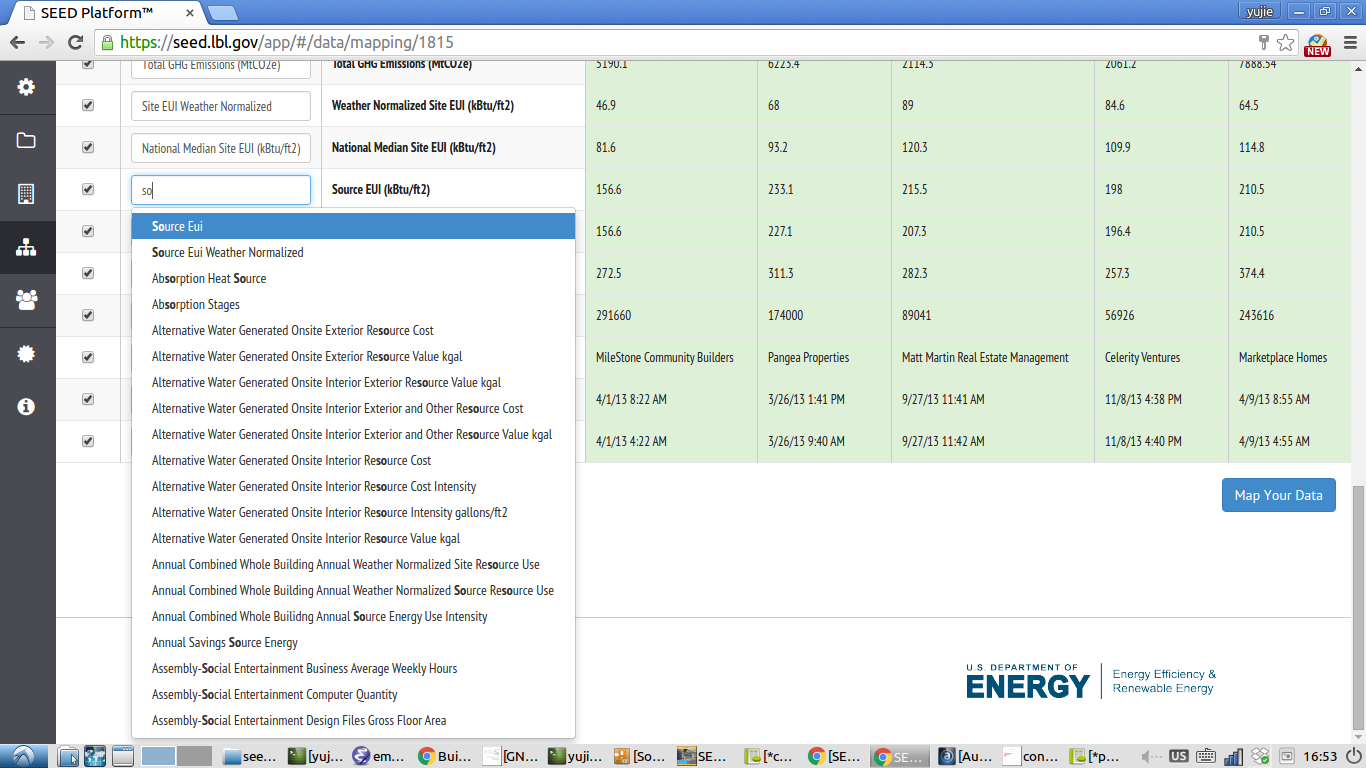
\includegraphics[width = 0.7\textwidth]{dropDown.png}
  \caption{Drop-down list for input BEDES term}~\cite{SEEDWebpage2015}
  \label{fig:dropDown}
\end{figure}

The guideline for the process is ``to improve results in matching
buildings across different data files, map as many of the following
four (4) fields as possible: Tax Lot ID, PM Property ID, Custom ID,
Address Line 1''~\cite{SEEDWebpage2015}.

\subsection{Matching} 

In this process the fields in the two input tables, the building list
and the PM data, are combined. The combining process utilizes some
common fields from the two tables. The process uses fuzzy string
searching~\cite{SEEDTutorial2015, approxStringMatchWiki} to auto map
the records in the two tables and returns a confidence score for the
matching. In the table below we can see the leading zeros does not
affect the matching result.

\begin{figure}[h!]
  \centering
  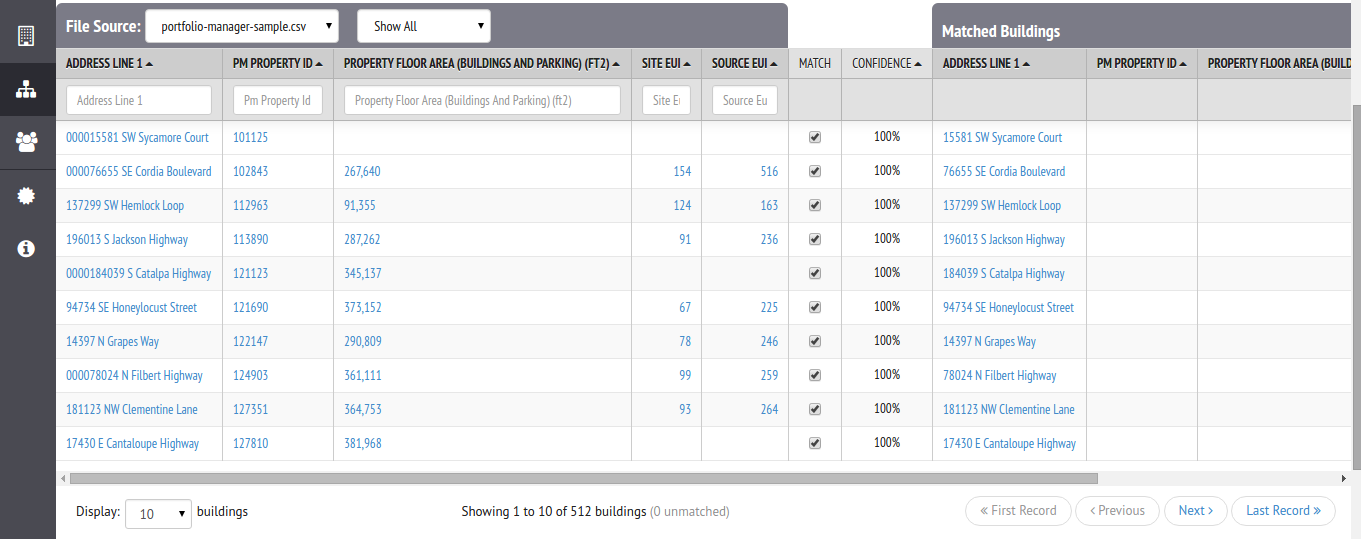
\includegraphics[width = 0.7\textwidth]{matchingResult.png}
  \caption{Matching result with confidence
    score}~\cite{SEEDWebpage2015}
  \label{fig:matchingResult}
\end{figure}

The matching can be manually corrected by clicking on the value of the
shared field in the source table and one can choose \textbf{one or
  more} records from the drop-down list that matches the record in the
source table (\fref{fig:matchManual}).

\begin{figure}[h!]
  \centering
  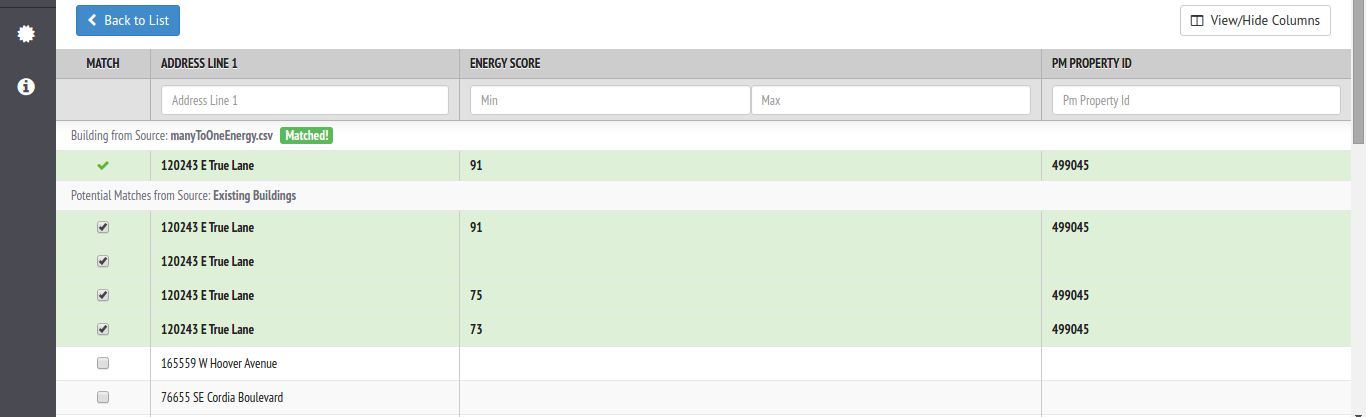
\includegraphics[width = 0.7\textwidth]{matchManual.png}
  \caption{Manually correct matching result by selecting one or more
    potential record}~\cite{SEEDWebpage2015}
  \label{fig:matchManual}
\end{figure}

In the matching process, one table is the source and the other is the
target. For each record/row in the target table, there is a unique
record in the source table that matches this record, a match will be
successful, but the score of confidence will not be 100\%. if there
are multiple records in the target that matches the source.

\begin{figure}[h!]
  \centering
  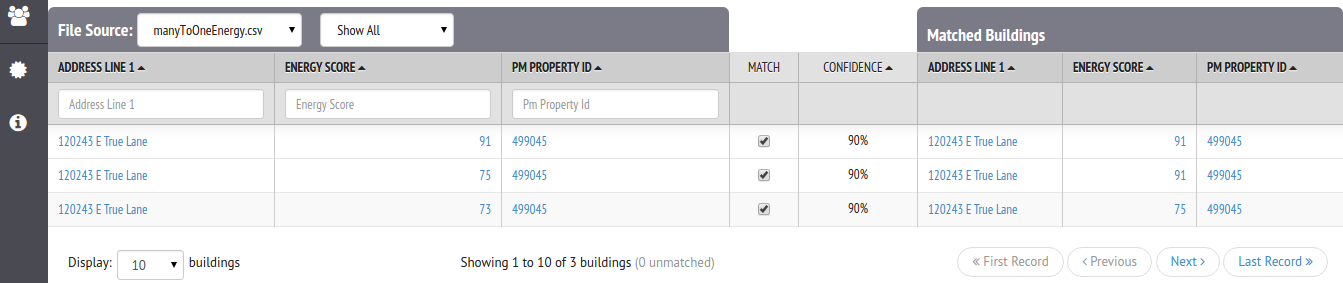
\includegraphics[width = 0.7\textwidth]{matchManyOne.png}
  \caption{Three records in the target table (PM table) matches one
    record in the source table (Building table)}~\cite{SEEDWebpage2015}
  \label{fig:matchManyOne}
\end{figure}

\section{Implementation strategy of mapping and matching: approximate
  string matching}
The approximate string matching aims at finding strings that
\emph{approximately} matches some pattern. The matching is normally
evaluated by some edit distance, which is the minimum number of
primitive operations (e.g. insertion, deletion and substitution)
needed to convert the approximate match to an exact
match~\cite{approxStringMatchWiki}. There are several versions of the
set of primitive operations. One common definition is the Levenshtein
distance, which include single character operations as insertion,
deletion and substitution.

There is a package in Python called FuzzyWuzzy~\cite{fuzzyWuzzy2015}
that evaluates the difference between strings with Levenshtein
distance. The package is built upon the Python package
\href{https://docs.python.org/2/library/difflib.html}{difflib} (which
has a class called ``SequenceMatcher'' that compares two sequences (
str, unicode, list, tuple, bytearray, buffer, xrange) as long as they
are hashable (those that can become a dictionary
key). \href{https://docs.python.org/2/glossary.html#term-immutable}{Immutable}
types (number, string, tuples) are all hashable in Python). There are
some explanation of the fuzzywuzzy package
\href{http://chairnerd.seatgeek.com/fuzzywuzzy-fuzzy-string-matching-in-python/}{here}. The
key functions include~\cite{fuzzyWuzzyGit2015}:
\makeatletter
\def\verbatim@font{\linespread{1}\small\ttfamily}
\makeatother
\begin{verbatim}
from fuzzywuzzy import fuzz
# simple ratio: pure edit distance
# similar to difflib.SequenceMatcher
fuzz.ratio("this is a test", "this is a test!")

# partial ratio: when s1 and s2 have very different lengths (WOLG, s1
< s2),
partial_ratio(s1, s2) returns fuzz.ratio(s1, s2') where s2' is a
sub string of s2 and len(s1) == len(s2')

fuzz.partial_ratio("this is a test", "this is a test!")

# token sort ratio: 
# to deal with the word re-order of strings
break strings to tokens, sort tokens and then re-assemble them to strings before calculating the ratio
fuzz.token_sort_ratio("fuzzy wuzzy was a bear", "wuzzy fuzzy was a bear")

# extracting a list of tuples of (str, score) where str is in choices 
# and score is the matching score between query and choice)
extract(query, choices, processor=None, scorer=None, limit=5)
\end{verbatim}

However, if the address line is selected as the field for matching
calculation, a \textbf{substitution of common abbreviations} should be
performed before the string searching process
(\href{http://citeseerx.ist.psu.edu/viewdoc/download?doi=10.1.1.119.714&rep=rep1&type=pdf}{Figure
  2 in this paper}).

Now I wrote a wrapper of matching function with fuzzywuzzy package,
next step is to know which field to match (address or not) find a set
of testing source and target strings to see if the matching function
works.

\newpage
\bibliographystyle{plain}
\bibliography{myCitation}
\end{document}